\documentclass[paper=a4, fontsize=9pt]{scrartcl}
\usepackage[bottom=0.9in, left=0.7in, right=0.7in, top=0.8in, foot=0.5in]{geometry}
\usepackage{layouts}

\usepackage[usenames,dvipsnames,x11names]{xcolor}

\usepackage[T1]{fontenc}
\usepackage{fourier}
\usepackage[english]{babel}
\usepackage{amsmath,amsfonts,amsthm}

\usepackage{sectsty}
\allsectionsfont{\centering \normalfont\scshape}

\usepackage{amssymb}
\usepackage{acronym}
\usepackage{booktabs}
\usepackage{caption}
\usepackage{fancyhdr}
\usepackage{float}
\usepackage{graphicx}
\usepackage[htt]{hyphenat}
\usepackage{lastpage}
\usepackage{multicol}
\usepackage{titlesec}
\usepackage[inline]{enumitem}
\usepackage{algorithm, algpseudocode}
\usepackage[export]{adjustbox}
\usepackage{pdflscape}

\usepackage{tikz}
\usepackage{pgfplots, pgfplotstable}
\pgfplotsset{compat=1.5}
\usepgfplotslibrary{colorbrewer}

\pagestyle{fancyplain}
\fancyhead{}
\fancyfoot[L]{}
\fancyfoot[C]{\thepage~of~4}
\renewcommand{\headrulewidth}{0pt}
\renewcommand{\footrulewidth}{0pt}
\setlength{\headheight}{13.6pt}

\newcommand{\horrule}[1]{\rule{\linewidth}{#1}}

\title{
\vspace{-1cm}
\normalfont \normalsize
\textsc{Norwegian University of Science and Technology\\IT3708 -- Bio-Inspired Artificial Intelligence}
\horrule{0.5pt} \\[0cm]
\Huge Project 4: Solving Job Shop Scheduling Problem\\Using Bio-Inspired Algorithms\\[-0.3cm]
\horrule{2pt} \\[0.1cm]
}

\newacro{JSSP}{Job-Shop Scheduling Problem}
\newacro{ACO}{Ant Colony Optimization}
\newacro{BA}{Bees Algorithm}
\newacro{PSO}{Particle Swarm Optimization}
\newacro{TS}{Taboo Search}

\author{Per Magnus Veierland\\permve@stud.ntnu.no}

\date{\normalsize\today}

\begin{document}

\maketitle

\setlength\columnsep{20pt}

\begin{multicols}{2}

% TODO Explain how schedules are built from solutions

% Representation of solutions (individual & chromosome) for each of the three algorithm representations. Using figure(s) for solution is a must. For each of the three algorithms, how do you build the schedule from respective solutions? (1.5p)

\section*{Schedule Representation}

All three optimizers utilize the same schedule representation as shown in Figure~\ref{figure:representation}. This representation is able to represent both infeasible and feasible solutions to the \ac{JSSP}. Depending on context in the implementation, this representation either represents the job preference for each machine in a solution, or it represents a solution to the \ac{JSSP} directly. For both the \ac{PSO} and the \ac{BA}, random individuals are generated as part of the search. This is done by building a schedule with a randomly permuted job ordering for each machine. If treated as a solution directly, such a solution may be infeasible as machines can deadlock. To ensure that all created solutions are feasible, each possibly infeasible solution is ``developed'' by treating the representation as a preference description. The G\&T~algorithm as described in \cite{sha2006hybrid} details how a preference description can be used to generate an active schedule which must be feasible.

The G\&T algorithm can be described in four steps:

\begin{enumerate}
    \item Initialize schedule $S=\varnothing$; $\Omega$ is initialized to contain all operations without job predecessors.
    \item Find $o^*=\arg \min_{o \in \Omega} f_o$, where $f_o$ is the earliest completion time for operation $o$; $f_o = s_o + p_o$, where $s_o$ is the earliest starting time for operation $o$, and $p_o$ is the processing time for operation $o$.
    \item \begin{enumerate}
        \item Identify conflict set $C = \{ o \in \Omega \vert m_o = m_{o^*} \land s_o < f_{o^*} \}$, where $m_o$ is the machine associated with $o$.
        \item Select $o \in C$ according to the preference specified in the encoded representation.
        \item Add $o$ to schedule $S$.
    \end{enumerate}
    \item If schedule $S$ is incomplete; remove $o$ from $\Omega$, add any immediate job successor of $o$ to $\Omega$, and continue from step~2.
\end{enumerate}

{
\vspace{0.3cm}
\centering
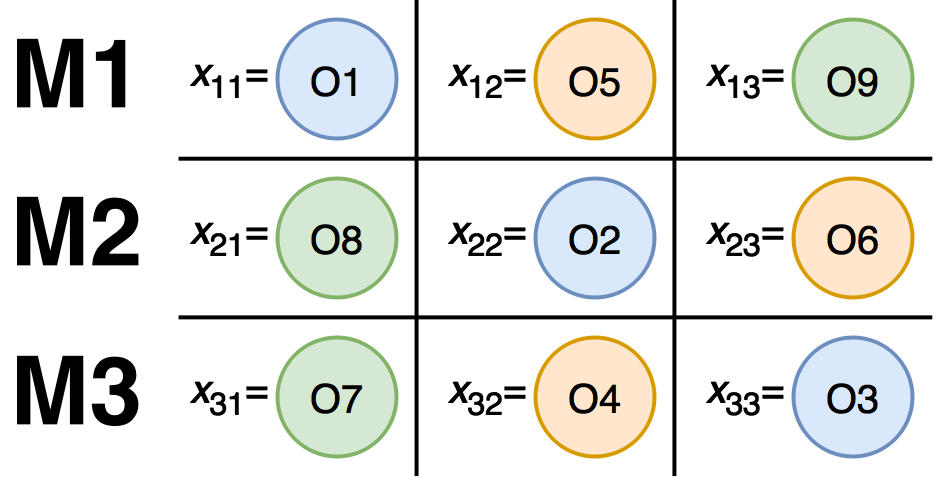
\includegraphics[scale=0.2]{figures/permve-ntnu-it3708-project-4-2017-schedule-representation}
\captionof{figure}{A \acs{JSSP} schedule is represented as an $m \times n$ matrix of $m$ machines and $n$ jobs. \textcolor{NavyBlue}{$\text{Job~1} = \langle\,\text{O}_1, \text{O}_2, \text{O}_3\,\rangle$}, \textcolor{Melon}{$\text{Job~2} = \langle\,\text{O}_4, \text{O}_5, \text{O}_6\rangle$}, \textcolor{OliveGreen}{$\text{Job~3} = \langle \text{O}_7, \text{O}_8, \text{O}_9\rangle$}. Each row $i$ encodes the ordering of operations for machine $i$; $M_1, M_2, M_3$.}
\label{figure:representation}
\vspace{0.3cm}
}

\section*{\acl{PSO}}

\acf{PSO} is an optimization technique mostly applied to problems with continuous solution spaces, where each particle in a swarm represents a solution. To solve a discrete problem such as \ac{JSSP}, inspiration has been taken from \cite{sha2006hybrid}. The resulting algorithm uses a discrete, preference-based representation, a modified approach velocity updates, a modified approach to position updates, a diversification strategy, and a local search. The overall algorithm can be described by the following three steps:

\begin{enumerate}
    \item The initial swarm population is generated, where the position of each particle $k$ is represented by a matrix of preferred machine operations $x^k$ as shown in Figure~\ref{figure:representation}. The job ordering for each machine is shuffled randomly, before the position of each particle $x^k$ is developed by the G\&T algorithm into a feasible schedule $S^k$.
    \item For each solution $S^k$ represented by particle $k$ in the swarm, its best historical schedule, as determined by the schedule makespan, is tracked as $\text{pbest}^k$. The best solution out of all particles is tracked as $\text{gbest}$.
    \item If the maximum number of iterations has not been reached:
    \begin{enumerate}
        \item Update the velocity $v^k$ for each particle $k$.
        \item For each particle $k$ in the swarm; update its position $x^k$ and develop the position $x^k$ into the schedule $S^k$. For each schedule $S^k$, apply \ac{TS}, before updating $\text{pbest}^k$ and $\text{gbest}$ accordingly.
    \end{enumerate}
\end{enumerate}

The velocity of each particle $k$ is represented by an $m \times n$ matrix, where the velocity of each operation $o_{ij}$ is denoted by $v_{ij} \in \{0,1\}$, and $o_{ij}$ is the operation of job~$j$ on machine~$i$. When $v_{ij}^k = 1$, the operation $o_{ij}$ of particle $k$ has just been moved to its current position in $x^k$, and cannot be moved. In this way, the adapted velocity mechanism imitates the behavior of continuous velocity by providing the discrete representation with momentum. The velocity $v_{ij}^k$ is randomly set to zero with a probability $(1-w)$ when updating the velocity of each particle.

{
\vspace{0.2cm}
\begin{minipage}{\linewidth{}}
\centering
\begin{tabular}{lc}
\toprule
Parameter                                   & Value \\
\midrule
Iterations                                  & 150   \\
Swarm size                                  & 100   \\
Particle best factor ($c_1$)                &   0.5 \\
Global best factor ($c_2$)                  &   0.3 \\
Probability of not resetting velocity ($w$) &   0.5 \\
\bottomrule
\end{tabular}
\captionof{table}{\acf{PSO} parameters.}
\label{table:psoparams}
\end{minipage}
}

Position updates relate to the discrete velocities. If $v_{ij}^k=0$, the operation $o_{ij}^k$ will be moved to the corresponding location of operation $o_{ij}^k$ in $\text{pbest}^k$ with probability $c_1$, or it will be moved to the corresponding location of $o_{ij}^k$ in $\text{gbest}$ with probability $c_2$. In this manner, the $\text{pbest}$ and $\text{gbest}$ solutions are used to guide the global \ac{PSO} search. The position update is performed as follows for each machine $i$:

\begin{enumerate}
    \item Randomly select a location $l$ in $x_i^k$.
    \item Denote the operation at location $l$ in $x_i^k$ by $O_1$.
    \item Find the location of operation $O_1$ in $\text{pbest}_i^k$ with probability $c_1$, or find the location of operation $O_1$ in $\text{gbest}_i$ with probability $c_2$. Denote the location found in $\text{pbest}_i^k$ or $\text{gbest}_i$ by $l'$, and denote the operation at location $l'$ in $x_i^k$ by $O_2$.
    \item If $O_2$ has been denoted, and the velocity components $v_{i{J_1}}^k$ and $v_{i{J_2}}^k$ for jobs $J_1$ and $J_2$, associated with operations $O_1$ and $O_2$, are both zero, then swap operations $O_1$ and $O_2$ in $x_i^k$, and set $v_{i{J_1}}^k \gets 1$.
    \item If all locations in $x_i^k$ has been considered, then the velocity update is completed. Otherwise, if $l<n$, set $l \gets l+1$, else assign $l \gets 1$, and continue from step~2.
\end{enumerate}

To prevent the \ac{PSO} search from getting stuck in local minima, a diversification strategy is used when updating $\text{pbest}^k$ and $\text{gbest}$. For each new solution $S^k$, the following update is used:

\begin{enumerate}
    \item If the makespan of $S^k$ is less than the makespan of $\text{gbest}$, set the $\text{pbest}$ solution with the worst makespan to the current $\text{gbest}$, and set $\text{gbest}$ to $S^k$.
    \item Otherwise, if the makespan of $S^k$ is equal to the makespan of any $\text{pbest}$ or the $\text{gbest}$ solution, replace the solution with the equal makespan with $S^k$.
    \item Otherwise, if the makespan of $S^k$ is better than the makespan of the worst $\text{pbest}$ solution, set the worst $\text{pbest}$ solution to $S^k$.
\end{enumerate}

The implemented \ac{PSO} uses Taboo search as described in \cite{nowicki1996fast} with backtracking and cycle detection. This local search, using parameters shown in Table~\ref{table:tsparams}, assists the global \ac{PSO} search aids the global \ac{PSO} search, which uses parameters shown in Table~\ref{table:psoparams}. The mutation operation described in \cite{sha2006hybrid} is not used.

\section*{\acl{ACO}}

\acf{ACO} is a swarm search inspired by how ants are able to locate food and direct other ants towards discovered food sources by using pheromones. The pheromone information is a central component in \ac{ACO} in guiding the search, by learning the relations between related operations as described in \cite{blum2004ant}. An operation $o_a$ is related to an operation $o_b$ if they are directly adjacent in a job sequence, or if they have to be processed by the same machine. The set of operations related to operation $o_a$ is denoted by $\mathcal{R}_a$.

The pheromone information is represented as an $\vert O \vert \times \vert O \vert$ matrix $\mathcal{T}$, where an entry $\mathcal{T}_{ab}$ represents the desirability of processing operation $o_a$ before operation $o_b$ with a specific value denoted by $\tau_{ab}$. Solutions are generated from the pheromone information using an algorithm similar to G\&T, with the exception of how the conflict set $C$ is chosen in step~3a, and how an operation is selected from $C$ in step~3b. This process will always generated feasible schedules.

In 50\% of cases, the conflict set is set to produce non-delay schedules; $C = \{o \in \Omega \vert s_o = \min_{o' \in \Omega} s_{o'}\}$. In the other cases, the conflict set is not limiting; $C = \Omega$.

The selection of an operation from the conflict set $C$ is done by drawing randomly according to the probabilities:

\begin{equation}
p(o_a \vert \mathcal{T}) = \frac
{
    \min_{o_b \in \mathcal{R}_a \cap O^{+}} \tau_{ab} \cdot \eta(o_a)^\beta
}
{
    \sum_{o_c \in C} \min_{o_b \in \mathcal{R}_a \cap O^{+}} \tau_{ab} \cdot \eta(o_a)^\beta
}, \quad \forall o_a \in C
\label{eq:acopoa}
\end{equation}

Where $O^{+}$ is the set of operations which has not yet been added to the schedule, and $\eta(o_a)$ is the heuristic information given by:

\begin{equation}
\eta(o_a) = \frac
{
    \frac{1}{s_{o_a} + 1}
}
{
    \sum_{o_c \in C} \frac{1}{s_{o_a} + 1}
}
\label{eq:acoheur}
\end{equation}

The \ac{ACO} search can be described by the following four operations, which are repeated for as long as necessary:

\begin{enumerate}
    \item Generate $n_a = \max \Big\{ 10, \big\lfloor \frac{\vert O \vert}{10} \big\rfloor \Big\}$ solutions to form the generation $\mathcal{G}$, using the G\&T algorithm with modified conflict set (Equation~\ref{eq:acopoa}) and selection (Equation~\ref{eq:acoheur}), where $n_a$ is the number of ants.
    \item Apply local search to improve each schedule in $\mathcal{G}$.
    \item Apply \ac{TS} to the schedule with the lowest makespan in $\mathcal{G}$.
    \item Update the pheromones according to Equation~\ref{eq:acophero}~and~\ref{eq:acodelta}, where $\eta$ is the rate of pheromone evaporation, and $S^{*}$ is the best schedule found by the \ac{ACO} search.
\end{enumerate}

\begin{equation}
\tau_{ab} \gets \tau_{ab} + \rho \cdot \big[ \delta(o_a, o_b) - \tau_{ab} \big]
\label{eq:acophero}
\end{equation}

\begin{equation}
\delta(o_a, o_b) =
\begin{cases}
1, \text{if $o_a$ is processed before $o_b$ in $S^{*}$}\\
0, \text{otherwise}
\end{cases}
\label{eq:acodelta}
\end{equation}

Pheromone values are limited to the range $[0.001, 0.999]$.

{
\vspace{0.2cm}
\begin{minipage}{\linewidth{}}
\centering
\begin{tabular}{lc}
\toprule
Parameter                                         & Value \\
\midrule
Iterations                                        & 20    \\
Heuristic power ($\beta$)                         & 10.0  \\
Evaporation rate ($\rho$)                         &  0.1  \\
Initial pheromone value ($\tau_{\text{initial}}$) &  0.5  \\
\bottomrule
\end{tabular}
\captionof{table}{\acf{ACO} parameters.}
\label{table:acoparams}
\end{minipage}
}


% construct solutions from pheromone info

% apply local search to each solution

% find best in iteration. apply taboo search

% update pheromones


\section*{\acl{BA}}

% TODO Figure explaining BA representation

\section*{\acl{TS}}

\bibliographystyle{unsrt}
\bibliography{references.bib}

{
\begin{minipage}{\linewidth{}}
\centering
\begin{tabular}{lc}
\toprule
Parameter                              & Value \\
\midrule
Iterations                             &  5 \\
Number of scouts ($n$)                 & 10 \\
Number of sites selected ($m$)         &  8 \\
Number of elite sites ($e$)            &  3 \\
Number of normal sites ($m-e$)         &  5 \\
Number of bees per elite site ($nep$)  &  1 \\
Number of bees per normal site ($nsp$) &  2 \\
\bottomrule
\end{tabular}
\captionof{table}{\acf{BA} parameters.}
\label{table:baparams}
\end{minipage}
}

{
\begin{minipage}{\linewidth{}}
\centering
\begin{tabular}{lc}
\toprule
Parameter                                             & Value \\
\midrule
Iteration limit (maxiter)                             &   150 \\
Total iteration limit ($\text{maxiter}_\text{total}$) &  1000 \\
Taboo list limit (maxt)                               &     5 \\
Backtracking limit (maxl)                             &     8 \\
Max cycle detection count ($\max c$)                  &     2 \\
Max cycle detection duration ($\max \delta$)          &   100 \\
\bottomrule
\end{tabular}
\captionof{table}{\acf{TS} parameters.}
\label{table:tsparams}
\end{minipage}
}

\end{multicols}

%\clearpage

% TODO Explain local search + figure

% For test problem #3, draw the gantt-chart targeting the best makespan. You need to draw for all three algorithms. (1.5p)

% \begin{landscape}
% {
% \begin{table}
% \hspace*{-0.5cm}
% \centering
% \begin{tabular}{l}
% 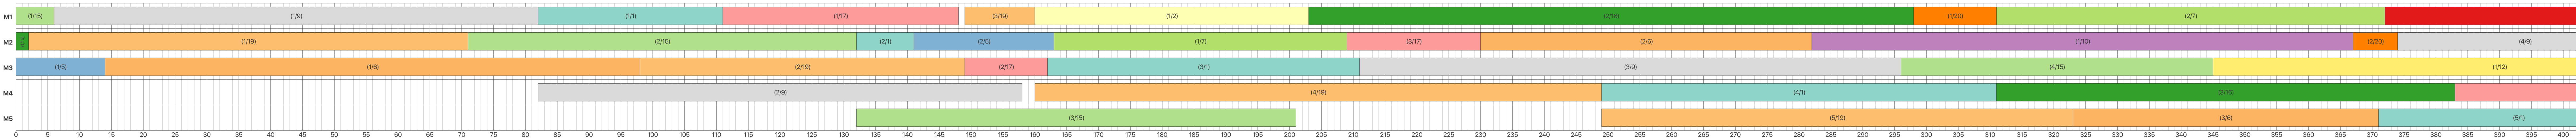
\includegraphics[height=40pt]{figures/solution_pso_instance_3_1_scaled}\\[0.15cm]
% \hspace{0.90909pt}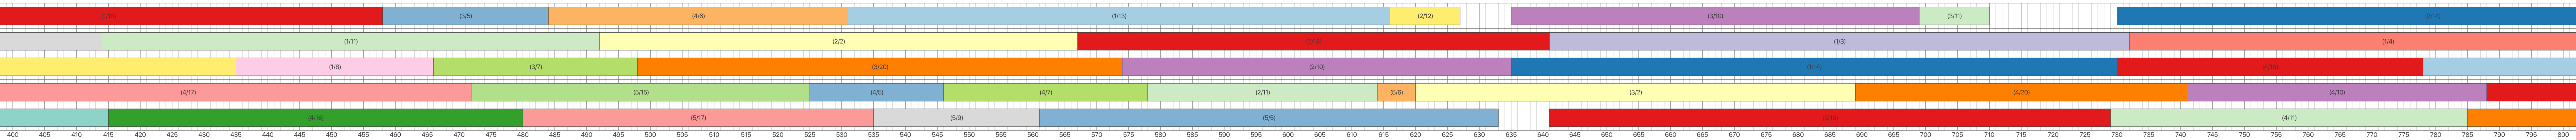
\includegraphics[height=40pt]{figures/solution_pso_instance_3_2_scaled}\\[0.15cm]
% \hspace{0.90909pt}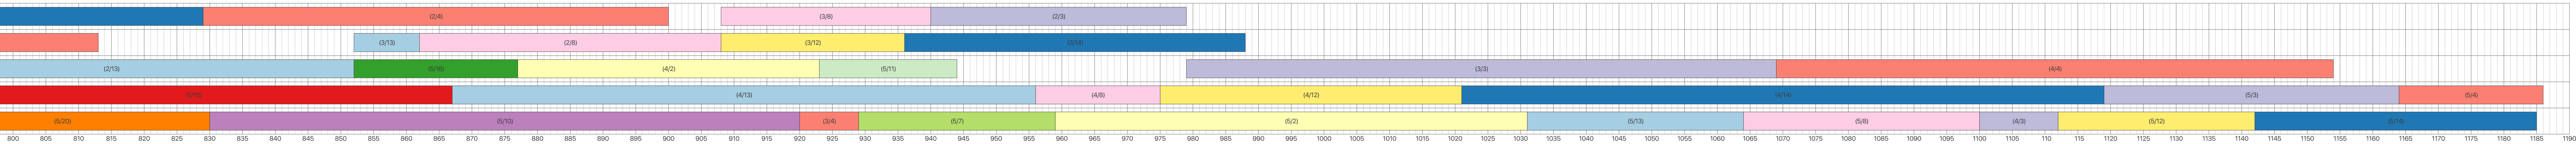
\includegraphics[height=40pt]{figures/solution_pso_instance_3_3_scaled}\\
% \multicolumn{1}{c}{\textit{Figure 1: \acf{PSO} solution with makespan 1186 for problem~3 using parameters specified in Table~\ref{table:psoparams}~and~\ref{table:tsparams}.}}\\[1.2cm]
% 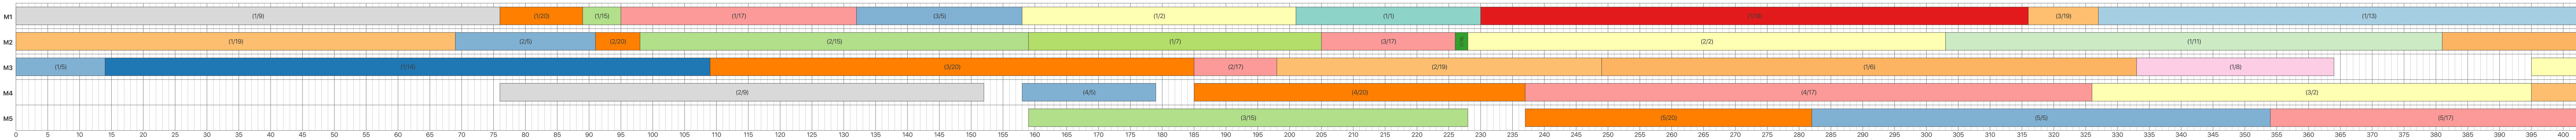
\includegraphics[height=40pt]{figures/solution_aco_instance_3_1_scaled}\\[0.15cm]
% \hspace{0.90909pt}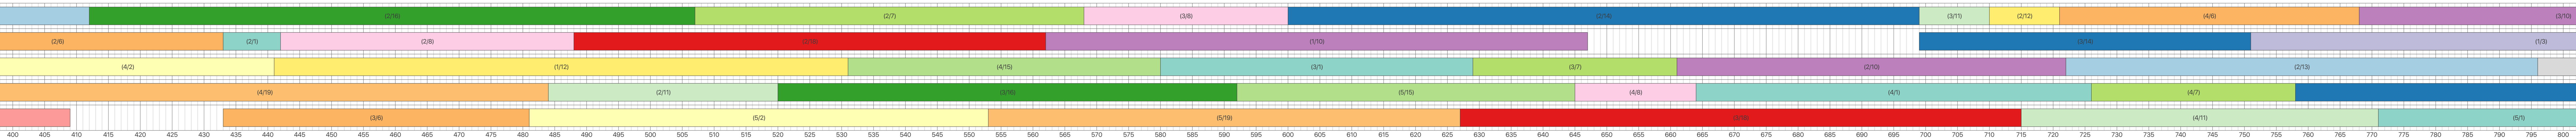
\includegraphics[height=40pt]{figures/solution_aco_instance_3_2_scaled}\\[0.15cm]
% \hspace{0.90909pt}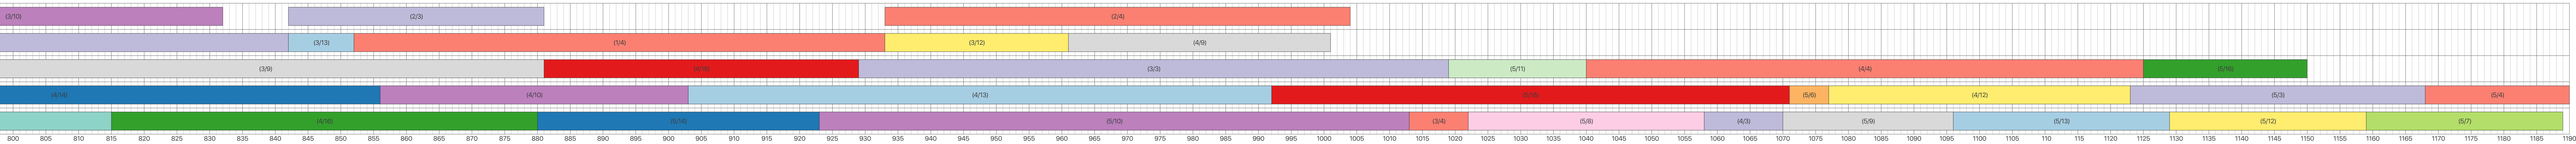
\includegraphics[height=40pt]{figures/solution_aco_instance_3_3_scaled}\\
% \multicolumn{1}{c}{\textit{Figure 2: \acf{ACO} solution with makespan 1190 for problem~3 using parameters specified in Table~\ref{table:acoparams}~and~\ref{table:tsparams}.}}\\[1.2cm]
% 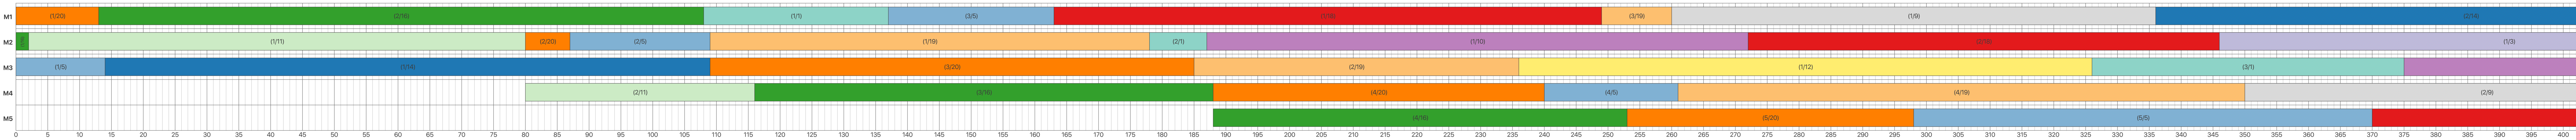
\includegraphics[height=40pt]{figures/solution_ba_instance_3_1_scaled}\\[0.15cm]
% \hspace{0.90909pt}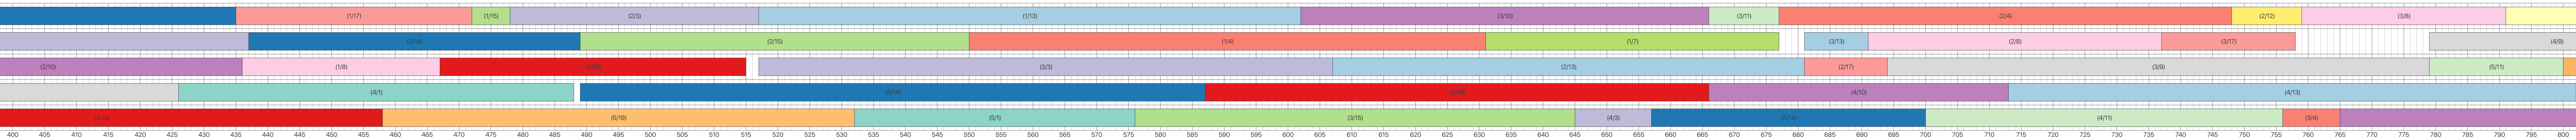
\includegraphics[height=40pt]{figures/solution_ba_instance_3_2_scaled}\\[0.15cm]
% \hspace{0.90909pt}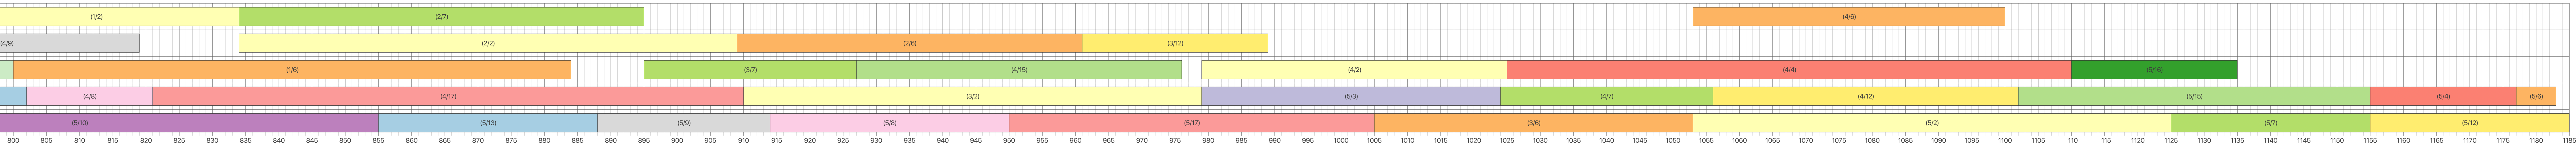
\includegraphics[height=40pt]{figures/solution_ba_instance_3_3_scaled}\\
% \multicolumn{1}{c}{\textit{Figure 3: \acf{BA} solution with makespan 1185 for problem~3 using parameters specified in Table~\ref{table:baparams}~and~\ref{table:tsparams}.}}\\
% \end{tabular}
% \end{table}
% }
% \end{landscape}

\end{document}
